\documentclass[
		book,
		head_space=20mm,
		foot_space=20mm,
		gutter=10mm,
		line_length=190mm
]{jlreq}

%----------
%LuaLaTeXで実行する!!
%----------
%各章節には以下を書く. 1-03.texのような名前にする
%----------
% \documentclass[
% 		book,
% 		head_space=20mm,
% 		foot_space=20mm,
% 		gutter=10mm,
% 		line_length=190mm
% ]{jlreq}
% 
%----------
%LuaLaTeXで実行する!!
%----------
%各章節には以下を書く. 1-03.texのような名前にする
%----------
% \documentclass[
% 		book,
% 		head_space=20mm,
% 		foot_space=20mm,
% 		gutter=10mm,
% 		line_length=190mm
% ]{jlreq}
% 
%----------
%LuaLaTeXで実行する!!
%----------
%各章節には以下を書く. 1-03.texのような名前にする
%----------
% \documentclass[
% 		book,
% 		head_space=20mm,
% 		foot_space=20mm,
% 		gutter=10mm,
% 		line_length=190mm
% ]{jlreq}
% \input {preamble.tex}
% \usepackage{docmute} %ファイル分割
% \begin{document}

% %\chapter{章のタイトル}
% \section{節のタイトル}
% no text

% \end{document}
%----------

%main.texには以下を書く
%----------
% \documentclass[
% 		book,
% 		head_space=20mm,
% 		foot_space=20mm,
% 		gutter=10mm,
% 		line_length=190mm,
%         openany
% ]{jlreq}
% \input {preamble.tex}
% \usepackage{docmute} %ファイル分割
% \begin{document}

% %---------- 1章1節
% \input 1-01.tex
% %---------- 1章2節
% \input 1-02.tex
% % ---------- 1章3節
% \input 1-03.tex
% % ---------- 1章4節
% \input 1-04.tex
% % ---------- 1章5節
% \input 1-05.tex
% % ---------- 1章6節
% \input 1-06.tex
% %---------- 1章7節
% \input 1-07.tex
% % ---------- 1章8節
% \input 1-08.tex
% % ---------- 1章9節
% \input 1-09.tex
% % ---------- 1章10節
% \input 1-10.tex
% % ---------- 1章11節
% \input 1-11.tex
% % ---------- 1章12節
% \input 1-12.tex
% % ---------- 参考文献
% \input reference.tex
% \end{document}
% ----------



\usepackage{bxtexlogo}
\usepackage{amsthm}
\usepackage{amsmath}
\usepackage{bbm} %小文字の黒板文字
\usepackage{physics}
\usepackage{amsfonts}
\usepackage{graphicx}
\usepackage{mathtools}
\usepackage{enumitem}
\usepackage[margin=20truemm]{geometry}
\usepackage{textcomp}
\usepackage{bm}
\usepackage{mathrsfs}
\usepackage{latexsym}
\usepackage{amssymb}
\usepackage{algorithmic}
\usepackage{algorithm}
\usepackage{tikz}
\usetikzlibrary{arrows.meta}
\usetikzlibrary{math,matrix,backgrounds}
\usetikzlibrary{angles}
\usetikzlibrary{calc}


%----------
%日本語フォント
% \usepackage[deluxe]{otf} platex用 lualatexでは動かない

%----------
%欧文フォント
\usepackage[T1]{fontenc}

%----------
%文字色
\usepackage{color}

%----------
\setlength{\parindent}{2\zw} %インデントの設定

%----------
% %参照した数式にだけ番号を振る cleverrefと併用するとうまくいかない
% \mathtoolsset{showonlyrefs=true}
%----------

%----------
%集合の中線
\newcommand{\relmiddle}[1]{\mathrel{}\middle#1\mathrel{}}
% \middle| の代わりに \relmiddle| を付ける
\newcommand{\sgn}{\mathop{\mathrm{sgn}}} %置換sgn
\newcommand{\Int}{\mathop{\mathrm{Int}}} %位相空間の内部Int
\newcommand{\Ext}{\mathop{\mathrm{Ext}}} %位相空間の外部Ext
\newcommand{\Cl}{\mathop{\mathrm{Cl}}} %位相空間の閉包Cl
\newcommand{\supp}{\mathop{\mathrm{supp}}} %関数の台supp
\newcommand{\restrict}[2]{\left. #1 \right \vert_{#2}}%関数の制限 \restrict{f}{A} = f|_A
\newcommand{\Ker}{\mathop{\mathrm{Ker}}}
\newcommand{\Coker}{\mathop{\mathrm{Coker}}}
\newcommand{\coker}{\mathop{\mathrm{coker}}}
\newcommand{\Coim}{\mathop{\mathrm{Coim}}}
\newcommand{\coim}{\mathop{\mathrm{coim}}}
\newcommand{\id}{\mathop{\mathrm{id}}}
\newcommand{\Gal}{\mathop{\mathrm{Gal}}}

\newtheorem{definition}{定義}[section]

\usepackage{aliascnt}

% \newaliastheorem{(環境とカウンターの名前)}{(元となるカウンターの名前)}{(表示される文字列)}
\newcommand*{\newaliastheorem}[3]{%
  \newaliascnt{#1}{#2}%
  \newtheorem{#1}[#1]{#3}%
  \aliascntresetthe{#1}%
  \expandafter\newcommand\csname #1autorefname\endcsname{#3}%
}
\newaliastheorem{proposition}{definition}{命題} 
\newaliastheorem{theorem}{definition}{定理}
\newaliastheorem{lemma}{definition}{補題}
\newaliastheorem{corollary}{definition}{系}
\newaliastheorem{example}{definition}{例}
\newaliastheorem{practice}{definition}{演習問題}

\newtheorem*{longproof}{証明}
\newtheorem*{answer}{解答}
\newtheorem*{supplement}{補足}
\newtheorem*{remark}{注意}
%----------

%----------
%古い記法を注意するパッケージ
\RequirePackage[l2tabu, orthodox]{nag}
%----------


% 定理環境(tcolorbox)
\usepackage{tcolorbox} %箱
\tcbuselibrary{breakable,skins,theorems}
\tcolorboxenvironment{definition}{
	blanker,breakable,
	left=3mm,right=3mm,
	top=2mm,bottom=2mm,
	before skip=15pt,after skip=20pt,
	borderline ={0.5pt}{0pt}{black}
}
\newtcolorbox{emptydefinition}{
	blanker,breakable,
	left=3mm,right=3mm,
	top=2mm,bottom=2mm,
	before skip=15pt,after skip=20pt,
	borderline ={0.5pt}{0pt}{black}
}
%----------
\tcolorboxenvironment{proposition}{
	blanker,breakable,
	left=3mm,right=3mm,
	top=3mm,bottom=3mm,
	before skip=15pt,after skip=15pt,
	borderline={0.5pt}{0pt}{black}
}
\newtcolorbox{emptyproposition}{
	blanker,breakable,
	left=3mm,right=3mm,
	top=3mm,bottom=3mm,
	before skip=15pt,after skip=15pt,
	borderline={0.5pt}{0pt}{black}
}
%----------
\tcolorboxenvironment{theorem}{
	blanker,breakable,
	left=3mm,right=3mm,
	top=3mm,bottom=3mm,
    sharp corners,boxrule=0.6pt,
	before skip=15pt,after skip=15pt,
	borderline={0.5pt}{0pt}{black},
    borderline={0.5pt}{1.5pt}{black}
}
\newtcolorbox{emptytheorem}{
	blanker,breakable,
	left=3mm,right=3mm,
	top=3mm,bottom=3mm,
    sharp corners,boxrule=0.6pt,
	before skip=15pt,after skip=15pt,
	borderline={0.5pt}{0pt}{black},
    borderline={0.5pt}{1.5pt}{black}
}
%----------
\tcolorboxenvironment{lemma}{
	blanker,breakable,
	left=3mm,right=3mm,
	top=3mm,bottom=3mm,
	before skip=15pt,after skip=15pt,
	borderline={0.5pt}{0pt}{black}
}
%----------
\tcolorboxenvironment{corollary}{
	blanker,breakable,
	left=3mm,right=3mm,
	top=3mm,bottom=3mm,
	before skip=15pt,after skip=15pt,
	borderline={1.0pt}{0pt}{black,dotted}
}
\newtcolorbox{emptycorollary}{
	blanker,breakable,
	left=3mm,right=3mm,
	top=3mm,bottom=3mm,
	before skip=15pt,after skip=15pt,
	borderline={1.0pt}{0pt}{black,dotted}
}
%----------
\tcolorboxenvironment{example}{
	blanker,breakable,
	left=3mm,right=3mm,
	top=3mm,bottom=3mm,
	before skip=15pt,after skip=15pt,
	borderline={0.5pt}{0pt}{black}
}
%----------
\tcolorboxenvironment{practice}{
	blanker,breakable,
	left=3mm,right=3mm,
	top=3mm,bottom=3mm,
	before skip=15pt,after skip=15pt,
	borderline={0.5pt}{0pt}{black}
}
%----------
\tcolorboxenvironment{proof}{
	blanker,breakable,
	left=3mm,right=3mm,
	top=2mm,bottom=2mm,
	before skip=15pt,after skip=20pt,
	% borderline west={1.5pt}{0pt}{black,dotted}
	borderline vertical={1pt}{0pt}{black,dotted}
	% borderline vertical={0.8pt}{0pt}{black,dotted,arrows={Square[scale=0.5]-Square[scale=0.5]}}
	}
%----------
\tcolorboxenvironment{supplement}{
	blanker,breakable,
	left=3mm,right=3mm,
	top=2mm,bottom=2mm,
	before skip=15pt,after skip=20pt,
	% borderline west={1.5pt}{0pt}{black,dotted}
	% borderline vertical={0.5pt}{0pt}{black,arrows = {Circle[scale=0.7]-Circle[scale=0.7]}}
	borderline vertical={0.5pt}{0pt}{black}
	% borderline vertical={0.5pt}{0pt}{black},
	% borderline north={0.5pt}{0pt}{white,arrows={Circle[black,scale=0.7]-Circle[black,scale=0.7]}}
	}
%----------
\tcolorboxenvironment{remark}{
	blanker,breakable,
	left=3mm,right=3mm,
	top=1mm,bottom=1mm,
	before skip=15pt,after skip=20pt,
	% borderline west={1.5pt}{0pt}{black,dotted}
	% borderline vertical={0.5pt}{0pt}{black,arrows = {Circle[scale=0.7]-Circle[scale=0.7]}}
	borderline vertical={0.5pt}{0pt}{black}
	% borderline vertical={0.5pt}{0pt}{black},
	% borderline north={0.5pt}{0pt}{white,arrows={Circle[black,scale=0.7]-Circle[black,scale=0.7]}}
	}
    
%---------------------
 

%----------
%ハイパーリンク
% 「%」は以降の内容を「改行コードも含めて」無視するコマンド
\usepackage[%
%  dvipdfmx,% 欧文ではコメントアウトする
luatex,%
pdfencoding=auto,%
 setpagesize=false,%
 bookmarks=true,%
 bookmarksdepth=tocdepth,%
 bookmarksnumbered=true,%
 colorlinks=false,%
 pdftitle={},%
 pdfsubject={},%
 pdfauthor={},%
 pdfkeywords={}%
]{hyperref}
%------------


%参照 参照するときに自動で環境名を含んで参照する
\usepackage[nameinlink]{cleveref}
\let\normalref\ref
\renewcommand{\ref}{\cref}
\crefname{definition}{定義}{定義}
\crefname{proposition}{命題}{命題}
\crefname{theorem}{定理}{定理}
\crefname{lemma}{補題}{補題}
\crefname{corollary}{系}{系}
\crefname{example}{例}{例}
\crefname{practice}{演習問題}{演習問題}
\crefname{equation}{式}{式} 
\crefname{chapter}{第}{第}
\creflabelformat{chapter}{#2#1章#3}
\crefname{section}{第}{第}
\creflabelformat{section}{#2#1節#3}
\crefname{subsection}{第}{第}
\creflabelformat{subsection}{#2#1小節#3}
%----------

%---------------------
%章跨ぎの参照が不具合を起こすための代わり
% \mylabl でラベル付け
\newcommand{\mylabel}[1]{
\label{#1}
\hypertarget{#1}{}
}
% \myref で環境名付きリンクをつける
\newcommand{\myref}[1]{
\hyperlink{#1}{\cref*{#1}}
}
%-----------------

\usepackage{autonum} %参照した数式にだけ番号を振る
% \usepackage{docmute} %ファイル分割
% \begin{document}

% %\chapter{章のタイトル}
% \section{節のタイトル}
% no text

% \end{document}
%----------

%main.texには以下を書く
%----------
% \documentclass[
% 		book,
% 		head_space=20mm,
% 		foot_space=20mm,
% 		gutter=10mm,
% 		line_length=190mm,
%         openany
% ]{jlreq}
% 
%----------
%LuaLaTeXで実行する!!
%----------
%各章節には以下を書く. 1-03.texのような名前にする
%----------
% \documentclass[
% 		book,
% 		head_space=20mm,
% 		foot_space=20mm,
% 		gutter=10mm,
% 		line_length=190mm
% ]{jlreq}
% \input {preamble.tex}
% \usepackage{docmute} %ファイル分割
% \begin{document}

% %\chapter{章のタイトル}
% \section{節のタイトル}
% no text

% \end{document}
%----------

%main.texには以下を書く
%----------
% \documentclass[
% 		book,
% 		head_space=20mm,
% 		foot_space=20mm,
% 		gutter=10mm,
% 		line_length=190mm,
%         openany
% ]{jlreq}
% \input {preamble.tex}
% \usepackage{docmute} %ファイル分割
% \begin{document}

% %---------- 1章1節
% \input 1-01.tex
% %---------- 1章2節
% \input 1-02.tex
% % ---------- 1章3節
% \input 1-03.tex
% % ---------- 1章4節
% \input 1-04.tex
% % ---------- 1章5節
% \input 1-05.tex
% % ---------- 1章6節
% \input 1-06.tex
% %---------- 1章7節
% \input 1-07.tex
% % ---------- 1章8節
% \input 1-08.tex
% % ---------- 1章9節
% \input 1-09.tex
% % ---------- 1章10節
% \input 1-10.tex
% % ---------- 1章11節
% \input 1-11.tex
% % ---------- 1章12節
% \input 1-12.tex
% % ---------- 参考文献
% \input reference.tex
% \end{document}
% ----------



\usepackage{bxtexlogo}
\usepackage{amsthm}
\usepackage{amsmath}
\usepackage{bbm} %小文字の黒板文字
\usepackage{physics}
\usepackage{amsfonts}
\usepackage{graphicx}
\usepackage{mathtools}
\usepackage{enumitem}
\usepackage[margin=20truemm]{geometry}
\usepackage{textcomp}
\usepackage{bm}
\usepackage{mathrsfs}
\usepackage{latexsym}
\usepackage{amssymb}
\usepackage{algorithmic}
\usepackage{algorithm}
\usepackage{tikz}
\usetikzlibrary{arrows.meta}
\usetikzlibrary{math,matrix,backgrounds}
\usetikzlibrary{angles}
\usetikzlibrary{calc}


%----------
%日本語フォント
% \usepackage[deluxe]{otf} platex用 lualatexでは動かない

%----------
%欧文フォント
\usepackage[T1]{fontenc}

%----------
%文字色
\usepackage{color}

%----------
\setlength{\parindent}{2\zw} %インデントの設定

%----------
% %参照した数式にだけ番号を振る cleverrefと併用するとうまくいかない
% \mathtoolsset{showonlyrefs=true}
%----------

%----------
%集合の中線
\newcommand{\relmiddle}[1]{\mathrel{}\middle#1\mathrel{}}
% \middle| の代わりに \relmiddle| を付ける
\newcommand{\sgn}{\mathop{\mathrm{sgn}}} %置換sgn
\newcommand{\Int}{\mathop{\mathrm{Int}}} %位相空間の内部Int
\newcommand{\Ext}{\mathop{\mathrm{Ext}}} %位相空間の外部Ext
\newcommand{\Cl}{\mathop{\mathrm{Cl}}} %位相空間の閉包Cl
\newcommand{\supp}{\mathop{\mathrm{supp}}} %関数の台supp
\newcommand{\restrict}[2]{\left. #1 \right \vert_{#2}}%関数の制限 \restrict{f}{A} = f|_A
\newcommand{\Ker}{\mathop{\mathrm{Ker}}}
\newcommand{\Coker}{\mathop{\mathrm{Coker}}}
\newcommand{\coker}{\mathop{\mathrm{coker}}}
\newcommand{\Coim}{\mathop{\mathrm{Coim}}}
\newcommand{\coim}{\mathop{\mathrm{coim}}}
\newcommand{\id}{\mathop{\mathrm{id}}}
\newcommand{\Gal}{\mathop{\mathrm{Gal}}}

\newtheorem{definition}{定義}[section]

\usepackage{aliascnt}

% \newaliastheorem{(環境とカウンターの名前)}{(元となるカウンターの名前)}{(表示される文字列)}
\newcommand*{\newaliastheorem}[3]{%
  \newaliascnt{#1}{#2}%
  \newtheorem{#1}[#1]{#3}%
  \aliascntresetthe{#1}%
  \expandafter\newcommand\csname #1autorefname\endcsname{#3}%
}
\newaliastheorem{proposition}{definition}{命題} 
\newaliastheorem{theorem}{definition}{定理}
\newaliastheorem{lemma}{definition}{補題}
\newaliastheorem{corollary}{definition}{系}
\newaliastheorem{example}{definition}{例}
\newaliastheorem{practice}{definition}{演習問題}

\newtheorem*{longproof}{証明}
\newtheorem*{answer}{解答}
\newtheorem*{supplement}{補足}
\newtheorem*{remark}{注意}
%----------

%----------
%古い記法を注意するパッケージ
\RequirePackage[l2tabu, orthodox]{nag}
%----------


% 定理環境(tcolorbox)
\usepackage{tcolorbox} %箱
\tcbuselibrary{breakable,skins,theorems}
\tcolorboxenvironment{definition}{
	blanker,breakable,
	left=3mm,right=3mm,
	top=2mm,bottom=2mm,
	before skip=15pt,after skip=20pt,
	borderline ={0.5pt}{0pt}{black}
}
\newtcolorbox{emptydefinition}{
	blanker,breakable,
	left=3mm,right=3mm,
	top=2mm,bottom=2mm,
	before skip=15pt,after skip=20pt,
	borderline ={0.5pt}{0pt}{black}
}
%----------
\tcolorboxenvironment{proposition}{
	blanker,breakable,
	left=3mm,right=3mm,
	top=3mm,bottom=3mm,
	before skip=15pt,after skip=15pt,
	borderline={0.5pt}{0pt}{black}
}
\newtcolorbox{emptyproposition}{
	blanker,breakable,
	left=3mm,right=3mm,
	top=3mm,bottom=3mm,
	before skip=15pt,after skip=15pt,
	borderline={0.5pt}{0pt}{black}
}
%----------
\tcolorboxenvironment{theorem}{
	blanker,breakable,
	left=3mm,right=3mm,
	top=3mm,bottom=3mm,
    sharp corners,boxrule=0.6pt,
	before skip=15pt,after skip=15pt,
	borderline={0.5pt}{0pt}{black},
    borderline={0.5pt}{1.5pt}{black}
}
\newtcolorbox{emptytheorem}{
	blanker,breakable,
	left=3mm,right=3mm,
	top=3mm,bottom=3mm,
    sharp corners,boxrule=0.6pt,
	before skip=15pt,after skip=15pt,
	borderline={0.5pt}{0pt}{black},
    borderline={0.5pt}{1.5pt}{black}
}
%----------
\tcolorboxenvironment{lemma}{
	blanker,breakable,
	left=3mm,right=3mm,
	top=3mm,bottom=3mm,
	before skip=15pt,after skip=15pt,
	borderline={0.5pt}{0pt}{black}
}
%----------
\tcolorboxenvironment{corollary}{
	blanker,breakable,
	left=3mm,right=3mm,
	top=3mm,bottom=3mm,
	before skip=15pt,after skip=15pt,
	borderline={1.0pt}{0pt}{black,dotted}
}
\newtcolorbox{emptycorollary}{
	blanker,breakable,
	left=3mm,right=3mm,
	top=3mm,bottom=3mm,
	before skip=15pt,after skip=15pt,
	borderline={1.0pt}{0pt}{black,dotted}
}
%----------
\tcolorboxenvironment{example}{
	blanker,breakable,
	left=3mm,right=3mm,
	top=3mm,bottom=3mm,
	before skip=15pt,after skip=15pt,
	borderline={0.5pt}{0pt}{black}
}
%----------
\tcolorboxenvironment{practice}{
	blanker,breakable,
	left=3mm,right=3mm,
	top=3mm,bottom=3mm,
	before skip=15pt,after skip=15pt,
	borderline={0.5pt}{0pt}{black}
}
%----------
\tcolorboxenvironment{proof}{
	blanker,breakable,
	left=3mm,right=3mm,
	top=2mm,bottom=2mm,
	before skip=15pt,after skip=20pt,
	% borderline west={1.5pt}{0pt}{black,dotted}
	borderline vertical={1pt}{0pt}{black,dotted}
	% borderline vertical={0.8pt}{0pt}{black,dotted,arrows={Square[scale=0.5]-Square[scale=0.5]}}
	}
%----------
\tcolorboxenvironment{supplement}{
	blanker,breakable,
	left=3mm,right=3mm,
	top=2mm,bottom=2mm,
	before skip=15pt,after skip=20pt,
	% borderline west={1.5pt}{0pt}{black,dotted}
	% borderline vertical={0.5pt}{0pt}{black,arrows = {Circle[scale=0.7]-Circle[scale=0.7]}}
	borderline vertical={0.5pt}{0pt}{black}
	% borderline vertical={0.5pt}{0pt}{black},
	% borderline north={0.5pt}{0pt}{white,arrows={Circle[black,scale=0.7]-Circle[black,scale=0.7]}}
	}
%----------
\tcolorboxenvironment{remark}{
	blanker,breakable,
	left=3mm,right=3mm,
	top=1mm,bottom=1mm,
	before skip=15pt,after skip=20pt,
	% borderline west={1.5pt}{0pt}{black,dotted}
	% borderline vertical={0.5pt}{0pt}{black,arrows = {Circle[scale=0.7]-Circle[scale=0.7]}}
	borderline vertical={0.5pt}{0pt}{black}
	% borderline vertical={0.5pt}{0pt}{black},
	% borderline north={0.5pt}{0pt}{white,arrows={Circle[black,scale=0.7]-Circle[black,scale=0.7]}}
	}
    
%---------------------
 

%----------
%ハイパーリンク
% 「%」は以降の内容を「改行コードも含めて」無視するコマンド
\usepackage[%
%  dvipdfmx,% 欧文ではコメントアウトする
luatex,%
pdfencoding=auto,%
 setpagesize=false,%
 bookmarks=true,%
 bookmarksdepth=tocdepth,%
 bookmarksnumbered=true,%
 colorlinks=false,%
 pdftitle={},%
 pdfsubject={},%
 pdfauthor={},%
 pdfkeywords={}%
]{hyperref}
%------------


%参照 参照するときに自動で環境名を含んで参照する
\usepackage[nameinlink]{cleveref}
\let\normalref\ref
\renewcommand{\ref}{\cref}
\crefname{definition}{定義}{定義}
\crefname{proposition}{命題}{命題}
\crefname{theorem}{定理}{定理}
\crefname{lemma}{補題}{補題}
\crefname{corollary}{系}{系}
\crefname{example}{例}{例}
\crefname{practice}{演習問題}{演習問題}
\crefname{equation}{式}{式} 
\crefname{chapter}{第}{第}
\creflabelformat{chapter}{#2#1章#3}
\crefname{section}{第}{第}
\creflabelformat{section}{#2#1節#3}
\crefname{subsection}{第}{第}
\creflabelformat{subsection}{#2#1小節#3}
%----------

%---------------------
%章跨ぎの参照が不具合を起こすための代わり
% \mylabl でラベル付け
\newcommand{\mylabel}[1]{
\label{#1}
\hypertarget{#1}{}
}
% \myref で環境名付きリンクをつける
\newcommand{\myref}[1]{
\hyperlink{#1}{\cref*{#1}}
}
%-----------------

\usepackage{autonum} %参照した数式にだけ番号を振る
% \usepackage{docmute} %ファイル分割
% \begin{document}

% %---------- 1章1節
% \input 1-01.tex
% %---------- 1章2節
% \input 1-02.tex
% % ---------- 1章3節
% \input 1-03.tex
% % ---------- 1章4節
% \input 1-04.tex
% % ---------- 1章5節
% \input 1-05.tex
% % ---------- 1章6節
% \input 1-06.tex
% %---------- 1章7節
% \input 1-07.tex
% % ---------- 1章8節
% \input 1-08.tex
% % ---------- 1章9節
% \input 1-09.tex
% % ---------- 1章10節
% \input 1-10.tex
% % ---------- 1章11節
% \input 1-11.tex
% % ---------- 1章12節
% \input 1-12.tex
% % ---------- 参考文献
% \input reference.tex
% \end{document}
% ----------



\usepackage{bxtexlogo}
\usepackage{amsthm}
\usepackage{amsmath}
\usepackage{bbm} %小文字の黒板文字
\usepackage{physics}
\usepackage{amsfonts}
\usepackage{graphicx}
\usepackage{mathtools}
\usepackage{enumitem}
\usepackage[margin=20truemm]{geometry}
\usepackage{textcomp}
\usepackage{bm}
\usepackage{mathrsfs}
\usepackage{latexsym}
\usepackage{amssymb}
\usepackage{algorithmic}
\usepackage{algorithm}
\usepackage{tikz}
\usetikzlibrary{arrows.meta}
\usetikzlibrary{math,matrix,backgrounds}
\usetikzlibrary{angles}
\usetikzlibrary{calc}


%----------
%日本語フォント
% \usepackage[deluxe]{otf} platex用 lualatexでは動かない

%----------
%欧文フォント
\usepackage[T1]{fontenc}

%----------
%文字色
\usepackage{color}

%----------
\setlength{\parindent}{2\zw} %インデントの設定

%----------
% %参照した数式にだけ番号を振る cleverrefと併用するとうまくいかない
% \mathtoolsset{showonlyrefs=true}
%----------

%----------
%集合の中線
\newcommand{\relmiddle}[1]{\mathrel{}\middle#1\mathrel{}}
% \middle| の代わりに \relmiddle| を付ける
\newcommand{\sgn}{\mathop{\mathrm{sgn}}} %置換sgn
\newcommand{\Int}{\mathop{\mathrm{Int}}} %位相空間の内部Int
\newcommand{\Ext}{\mathop{\mathrm{Ext}}} %位相空間の外部Ext
\newcommand{\Cl}{\mathop{\mathrm{Cl}}} %位相空間の閉包Cl
\newcommand{\supp}{\mathop{\mathrm{supp}}} %関数の台supp
\newcommand{\restrict}[2]{\left. #1 \right \vert_{#2}}%関数の制限 \restrict{f}{A} = f|_A
\newcommand{\Ker}{\mathop{\mathrm{Ker}}}
\newcommand{\Coker}{\mathop{\mathrm{Coker}}}
\newcommand{\coker}{\mathop{\mathrm{coker}}}
\newcommand{\Coim}{\mathop{\mathrm{Coim}}}
\newcommand{\coim}{\mathop{\mathrm{coim}}}
\newcommand{\id}{\mathop{\mathrm{id}}}
\newcommand{\Gal}{\mathop{\mathrm{Gal}}}

\newtheorem{definition}{定義}[section]

\usepackage{aliascnt}

% \newaliastheorem{(環境とカウンターの名前)}{(元となるカウンターの名前)}{(表示される文字列)}
\newcommand*{\newaliastheorem}[3]{%
  \newaliascnt{#1}{#2}%
  \newtheorem{#1}[#1]{#3}%
  \aliascntresetthe{#1}%
  \expandafter\newcommand\csname #1autorefname\endcsname{#3}%
}
\newaliastheorem{proposition}{definition}{命題} 
\newaliastheorem{theorem}{definition}{定理}
\newaliastheorem{lemma}{definition}{補題}
\newaliastheorem{corollary}{definition}{系}
\newaliastheorem{example}{definition}{例}
\newaliastheorem{practice}{definition}{演習問題}

\newtheorem*{longproof}{証明}
\newtheorem*{answer}{解答}
\newtheorem*{supplement}{補足}
\newtheorem*{remark}{注意}
%----------

%----------
%古い記法を注意するパッケージ
\RequirePackage[l2tabu, orthodox]{nag}
%----------


% 定理環境(tcolorbox)
\usepackage{tcolorbox} %箱
\tcbuselibrary{breakable,skins,theorems}
\tcolorboxenvironment{definition}{
	blanker,breakable,
	left=3mm,right=3mm,
	top=2mm,bottom=2mm,
	before skip=15pt,after skip=20pt,
	borderline ={0.5pt}{0pt}{black}
}
\newtcolorbox{emptydefinition}{
	blanker,breakable,
	left=3mm,right=3mm,
	top=2mm,bottom=2mm,
	before skip=15pt,after skip=20pt,
	borderline ={0.5pt}{0pt}{black}
}
%----------
\tcolorboxenvironment{proposition}{
	blanker,breakable,
	left=3mm,right=3mm,
	top=3mm,bottom=3mm,
	before skip=15pt,after skip=15pt,
	borderline={0.5pt}{0pt}{black}
}
\newtcolorbox{emptyproposition}{
	blanker,breakable,
	left=3mm,right=3mm,
	top=3mm,bottom=3mm,
	before skip=15pt,after skip=15pt,
	borderline={0.5pt}{0pt}{black}
}
%----------
\tcolorboxenvironment{theorem}{
	blanker,breakable,
	left=3mm,right=3mm,
	top=3mm,bottom=3mm,
    sharp corners,boxrule=0.6pt,
	before skip=15pt,after skip=15pt,
	borderline={0.5pt}{0pt}{black},
    borderline={0.5pt}{1.5pt}{black}
}
\newtcolorbox{emptytheorem}{
	blanker,breakable,
	left=3mm,right=3mm,
	top=3mm,bottom=3mm,
    sharp corners,boxrule=0.6pt,
	before skip=15pt,after skip=15pt,
	borderline={0.5pt}{0pt}{black},
    borderline={0.5pt}{1.5pt}{black}
}
%----------
\tcolorboxenvironment{lemma}{
	blanker,breakable,
	left=3mm,right=3mm,
	top=3mm,bottom=3mm,
	before skip=15pt,after skip=15pt,
	borderline={0.5pt}{0pt}{black}
}
%----------
\tcolorboxenvironment{corollary}{
	blanker,breakable,
	left=3mm,right=3mm,
	top=3mm,bottom=3mm,
	before skip=15pt,after skip=15pt,
	borderline={1.0pt}{0pt}{black,dotted}
}
\newtcolorbox{emptycorollary}{
	blanker,breakable,
	left=3mm,right=3mm,
	top=3mm,bottom=3mm,
	before skip=15pt,after skip=15pt,
	borderline={1.0pt}{0pt}{black,dotted}
}
%----------
\tcolorboxenvironment{example}{
	blanker,breakable,
	left=3mm,right=3mm,
	top=3mm,bottom=3mm,
	before skip=15pt,after skip=15pt,
	borderline={0.5pt}{0pt}{black}
}
%----------
\tcolorboxenvironment{practice}{
	blanker,breakable,
	left=3mm,right=3mm,
	top=3mm,bottom=3mm,
	before skip=15pt,after skip=15pt,
	borderline={0.5pt}{0pt}{black}
}
%----------
\tcolorboxenvironment{proof}{
	blanker,breakable,
	left=3mm,right=3mm,
	top=2mm,bottom=2mm,
	before skip=15pt,after skip=20pt,
	% borderline west={1.5pt}{0pt}{black,dotted}
	borderline vertical={1pt}{0pt}{black,dotted}
	% borderline vertical={0.8pt}{0pt}{black,dotted,arrows={Square[scale=0.5]-Square[scale=0.5]}}
	}
%----------
\tcolorboxenvironment{supplement}{
	blanker,breakable,
	left=3mm,right=3mm,
	top=2mm,bottom=2mm,
	before skip=15pt,after skip=20pt,
	% borderline west={1.5pt}{0pt}{black,dotted}
	% borderline vertical={0.5pt}{0pt}{black,arrows = {Circle[scale=0.7]-Circle[scale=0.7]}}
	borderline vertical={0.5pt}{0pt}{black}
	% borderline vertical={0.5pt}{0pt}{black},
	% borderline north={0.5pt}{0pt}{white,arrows={Circle[black,scale=0.7]-Circle[black,scale=0.7]}}
	}
%----------
\tcolorboxenvironment{remark}{
	blanker,breakable,
	left=3mm,right=3mm,
	top=1mm,bottom=1mm,
	before skip=15pt,after skip=20pt,
	% borderline west={1.5pt}{0pt}{black,dotted}
	% borderline vertical={0.5pt}{0pt}{black,arrows = {Circle[scale=0.7]-Circle[scale=0.7]}}
	borderline vertical={0.5pt}{0pt}{black}
	% borderline vertical={0.5pt}{0pt}{black},
	% borderline north={0.5pt}{0pt}{white,arrows={Circle[black,scale=0.7]-Circle[black,scale=0.7]}}
	}
    
%---------------------
 

%----------
%ハイパーリンク
% 「%」は以降の内容を「改行コードも含めて」無視するコマンド
\usepackage[%
%  dvipdfmx,% 欧文ではコメントアウトする
luatex,%
pdfencoding=auto,%
 setpagesize=false,%
 bookmarks=true,%
 bookmarksdepth=tocdepth,%
 bookmarksnumbered=true,%
 colorlinks=false,%
 pdftitle={},%
 pdfsubject={},%
 pdfauthor={},%
 pdfkeywords={}%
]{hyperref}
%------------


%参照 参照するときに自動で環境名を含んで参照する
\usepackage[nameinlink]{cleveref}
\let\normalref\ref
\renewcommand{\ref}{\cref}
\crefname{definition}{定義}{定義}
\crefname{proposition}{命題}{命題}
\crefname{theorem}{定理}{定理}
\crefname{lemma}{補題}{補題}
\crefname{corollary}{系}{系}
\crefname{example}{例}{例}
\crefname{practice}{演習問題}{演習問題}
\crefname{equation}{式}{式} 
\crefname{chapter}{第}{第}
\creflabelformat{chapter}{#2#1章#3}
\crefname{section}{第}{第}
\creflabelformat{section}{#2#1節#3}
\crefname{subsection}{第}{第}
\creflabelformat{subsection}{#2#1小節#3}
%----------

%---------------------
%章跨ぎの参照が不具合を起こすための代わり
% \mylabl でラベル付け
\newcommand{\mylabel}[1]{
\label{#1}
\hypertarget{#1}{}
}
% \myref で環境名付きリンクをつける
\newcommand{\myref}[1]{
\hyperlink{#1}{\cref*{#1}}
}
%-----------------

\usepackage{autonum} %参照した数式にだけ番号を振る
% \usepackage{docmute} %ファイル分割
% \begin{document}

% %\chapter{章のタイトル}
% \section{節のタイトル}
% no text

% \end{document}
%----------

%main.texには以下を書く
%----------
% \documentclass[
% 		book,
% 		head_space=20mm,
% 		foot_space=20mm,
% 		gutter=10mm,
% 		line_length=190mm,
%         openany
% ]{jlreq}
% 
%----------
%LuaLaTeXで実行する!!
%----------
%各章節には以下を書く. 1-03.texのような名前にする
%----------
% \documentclass[
% 		book,
% 		head_space=20mm,
% 		foot_space=20mm,
% 		gutter=10mm,
% 		line_length=190mm
% ]{jlreq}
% 
%----------
%LuaLaTeXで実行する!!
%----------
%各章節には以下を書く. 1-03.texのような名前にする
%----------
% \documentclass[
% 		book,
% 		head_space=20mm,
% 		foot_space=20mm,
% 		gutter=10mm,
% 		line_length=190mm
% ]{jlreq}
% \input {preamble.tex}
% \usepackage{docmute} %ファイル分割
% \begin{document}

% %\chapter{章のタイトル}
% \section{節のタイトル}
% no text

% \end{document}
%----------

%main.texには以下を書く
%----------
% \documentclass[
% 		book,
% 		head_space=20mm,
% 		foot_space=20mm,
% 		gutter=10mm,
% 		line_length=190mm,
%         openany
% ]{jlreq}
% \input {preamble.tex}
% \usepackage{docmute} %ファイル分割
% \begin{document}

% %---------- 1章1節
% \input 1-01.tex
% %---------- 1章2節
% \input 1-02.tex
% % ---------- 1章3節
% \input 1-03.tex
% % ---------- 1章4節
% \input 1-04.tex
% % ---------- 1章5節
% \input 1-05.tex
% % ---------- 1章6節
% \input 1-06.tex
% %---------- 1章7節
% \input 1-07.tex
% % ---------- 1章8節
% \input 1-08.tex
% % ---------- 1章9節
% \input 1-09.tex
% % ---------- 1章10節
% \input 1-10.tex
% % ---------- 1章11節
% \input 1-11.tex
% % ---------- 1章12節
% \input 1-12.tex
% % ---------- 参考文献
% \input reference.tex
% \end{document}
% ----------



\usepackage{bxtexlogo}
\usepackage{amsthm}
\usepackage{amsmath}
\usepackage{bbm} %小文字の黒板文字
\usepackage{physics}
\usepackage{amsfonts}
\usepackage{graphicx}
\usepackage{mathtools}
\usepackage{enumitem}
\usepackage[margin=20truemm]{geometry}
\usepackage{textcomp}
\usepackage{bm}
\usepackage{mathrsfs}
\usepackage{latexsym}
\usepackage{amssymb}
\usepackage{algorithmic}
\usepackage{algorithm}
\usepackage{tikz}
\usetikzlibrary{arrows.meta}
\usetikzlibrary{math,matrix,backgrounds}
\usetikzlibrary{angles}
\usetikzlibrary{calc}


%----------
%日本語フォント
% \usepackage[deluxe]{otf} platex用 lualatexでは動かない

%----------
%欧文フォント
\usepackage[T1]{fontenc}

%----------
%文字色
\usepackage{color}

%----------
\setlength{\parindent}{2\zw} %インデントの設定

%----------
% %参照した数式にだけ番号を振る cleverrefと併用するとうまくいかない
% \mathtoolsset{showonlyrefs=true}
%----------

%----------
%集合の中線
\newcommand{\relmiddle}[1]{\mathrel{}\middle#1\mathrel{}}
% \middle| の代わりに \relmiddle| を付ける
\newcommand{\sgn}{\mathop{\mathrm{sgn}}} %置換sgn
\newcommand{\Int}{\mathop{\mathrm{Int}}} %位相空間の内部Int
\newcommand{\Ext}{\mathop{\mathrm{Ext}}} %位相空間の外部Ext
\newcommand{\Cl}{\mathop{\mathrm{Cl}}} %位相空間の閉包Cl
\newcommand{\supp}{\mathop{\mathrm{supp}}} %関数の台supp
\newcommand{\restrict}[2]{\left. #1 \right \vert_{#2}}%関数の制限 \restrict{f}{A} = f|_A
\newcommand{\Ker}{\mathop{\mathrm{Ker}}}
\newcommand{\Coker}{\mathop{\mathrm{Coker}}}
\newcommand{\coker}{\mathop{\mathrm{coker}}}
\newcommand{\Coim}{\mathop{\mathrm{Coim}}}
\newcommand{\coim}{\mathop{\mathrm{coim}}}
\newcommand{\id}{\mathop{\mathrm{id}}}
\newcommand{\Gal}{\mathop{\mathrm{Gal}}}

\newtheorem{definition}{定義}[section]

\usepackage{aliascnt}

% \newaliastheorem{(環境とカウンターの名前)}{(元となるカウンターの名前)}{(表示される文字列)}
\newcommand*{\newaliastheorem}[3]{%
  \newaliascnt{#1}{#2}%
  \newtheorem{#1}[#1]{#3}%
  \aliascntresetthe{#1}%
  \expandafter\newcommand\csname #1autorefname\endcsname{#3}%
}
\newaliastheorem{proposition}{definition}{命題} 
\newaliastheorem{theorem}{definition}{定理}
\newaliastheorem{lemma}{definition}{補題}
\newaliastheorem{corollary}{definition}{系}
\newaliastheorem{example}{definition}{例}
\newaliastheorem{practice}{definition}{演習問題}

\newtheorem*{longproof}{証明}
\newtheorem*{answer}{解答}
\newtheorem*{supplement}{補足}
\newtheorem*{remark}{注意}
%----------

%----------
%古い記法を注意するパッケージ
\RequirePackage[l2tabu, orthodox]{nag}
%----------


% 定理環境(tcolorbox)
\usepackage{tcolorbox} %箱
\tcbuselibrary{breakable,skins,theorems}
\tcolorboxenvironment{definition}{
	blanker,breakable,
	left=3mm,right=3mm,
	top=2mm,bottom=2mm,
	before skip=15pt,after skip=20pt,
	borderline ={0.5pt}{0pt}{black}
}
\newtcolorbox{emptydefinition}{
	blanker,breakable,
	left=3mm,right=3mm,
	top=2mm,bottom=2mm,
	before skip=15pt,after skip=20pt,
	borderline ={0.5pt}{0pt}{black}
}
%----------
\tcolorboxenvironment{proposition}{
	blanker,breakable,
	left=3mm,right=3mm,
	top=3mm,bottom=3mm,
	before skip=15pt,after skip=15pt,
	borderline={0.5pt}{0pt}{black}
}
\newtcolorbox{emptyproposition}{
	blanker,breakable,
	left=3mm,right=3mm,
	top=3mm,bottom=3mm,
	before skip=15pt,after skip=15pt,
	borderline={0.5pt}{0pt}{black}
}
%----------
\tcolorboxenvironment{theorem}{
	blanker,breakable,
	left=3mm,right=3mm,
	top=3mm,bottom=3mm,
    sharp corners,boxrule=0.6pt,
	before skip=15pt,after skip=15pt,
	borderline={0.5pt}{0pt}{black},
    borderline={0.5pt}{1.5pt}{black}
}
\newtcolorbox{emptytheorem}{
	blanker,breakable,
	left=3mm,right=3mm,
	top=3mm,bottom=3mm,
    sharp corners,boxrule=0.6pt,
	before skip=15pt,after skip=15pt,
	borderline={0.5pt}{0pt}{black},
    borderline={0.5pt}{1.5pt}{black}
}
%----------
\tcolorboxenvironment{lemma}{
	blanker,breakable,
	left=3mm,right=3mm,
	top=3mm,bottom=3mm,
	before skip=15pt,after skip=15pt,
	borderline={0.5pt}{0pt}{black}
}
%----------
\tcolorboxenvironment{corollary}{
	blanker,breakable,
	left=3mm,right=3mm,
	top=3mm,bottom=3mm,
	before skip=15pt,after skip=15pt,
	borderline={1.0pt}{0pt}{black,dotted}
}
\newtcolorbox{emptycorollary}{
	blanker,breakable,
	left=3mm,right=3mm,
	top=3mm,bottom=3mm,
	before skip=15pt,after skip=15pt,
	borderline={1.0pt}{0pt}{black,dotted}
}
%----------
\tcolorboxenvironment{example}{
	blanker,breakable,
	left=3mm,right=3mm,
	top=3mm,bottom=3mm,
	before skip=15pt,after skip=15pt,
	borderline={0.5pt}{0pt}{black}
}
%----------
\tcolorboxenvironment{practice}{
	blanker,breakable,
	left=3mm,right=3mm,
	top=3mm,bottom=3mm,
	before skip=15pt,after skip=15pt,
	borderline={0.5pt}{0pt}{black}
}
%----------
\tcolorboxenvironment{proof}{
	blanker,breakable,
	left=3mm,right=3mm,
	top=2mm,bottom=2mm,
	before skip=15pt,after skip=20pt,
	% borderline west={1.5pt}{0pt}{black,dotted}
	borderline vertical={1pt}{0pt}{black,dotted}
	% borderline vertical={0.8pt}{0pt}{black,dotted,arrows={Square[scale=0.5]-Square[scale=0.5]}}
	}
%----------
\tcolorboxenvironment{supplement}{
	blanker,breakable,
	left=3mm,right=3mm,
	top=2mm,bottom=2mm,
	before skip=15pt,after skip=20pt,
	% borderline west={1.5pt}{0pt}{black,dotted}
	% borderline vertical={0.5pt}{0pt}{black,arrows = {Circle[scale=0.7]-Circle[scale=0.7]}}
	borderline vertical={0.5pt}{0pt}{black}
	% borderline vertical={0.5pt}{0pt}{black},
	% borderline north={0.5pt}{0pt}{white,arrows={Circle[black,scale=0.7]-Circle[black,scale=0.7]}}
	}
%----------
\tcolorboxenvironment{remark}{
	blanker,breakable,
	left=3mm,right=3mm,
	top=1mm,bottom=1mm,
	before skip=15pt,after skip=20pt,
	% borderline west={1.5pt}{0pt}{black,dotted}
	% borderline vertical={0.5pt}{0pt}{black,arrows = {Circle[scale=0.7]-Circle[scale=0.7]}}
	borderline vertical={0.5pt}{0pt}{black}
	% borderline vertical={0.5pt}{0pt}{black},
	% borderline north={0.5pt}{0pt}{white,arrows={Circle[black,scale=0.7]-Circle[black,scale=0.7]}}
	}
    
%---------------------
 

%----------
%ハイパーリンク
% 「%」は以降の内容を「改行コードも含めて」無視するコマンド
\usepackage[%
%  dvipdfmx,% 欧文ではコメントアウトする
luatex,%
pdfencoding=auto,%
 setpagesize=false,%
 bookmarks=true,%
 bookmarksdepth=tocdepth,%
 bookmarksnumbered=true,%
 colorlinks=false,%
 pdftitle={},%
 pdfsubject={},%
 pdfauthor={},%
 pdfkeywords={}%
]{hyperref}
%------------


%参照 参照するときに自動で環境名を含んで参照する
\usepackage[nameinlink]{cleveref}
\let\normalref\ref
\renewcommand{\ref}{\cref}
\crefname{definition}{定義}{定義}
\crefname{proposition}{命題}{命題}
\crefname{theorem}{定理}{定理}
\crefname{lemma}{補題}{補題}
\crefname{corollary}{系}{系}
\crefname{example}{例}{例}
\crefname{practice}{演習問題}{演習問題}
\crefname{equation}{式}{式} 
\crefname{chapter}{第}{第}
\creflabelformat{chapter}{#2#1章#3}
\crefname{section}{第}{第}
\creflabelformat{section}{#2#1節#3}
\crefname{subsection}{第}{第}
\creflabelformat{subsection}{#2#1小節#3}
%----------

%---------------------
%章跨ぎの参照が不具合を起こすための代わり
% \mylabl でラベル付け
\newcommand{\mylabel}[1]{
\label{#1}
\hypertarget{#1}{}
}
% \myref で環境名付きリンクをつける
\newcommand{\myref}[1]{
\hyperlink{#1}{\cref*{#1}}
}
%-----------------

\usepackage{autonum} %参照した数式にだけ番号を振る
% \usepackage{docmute} %ファイル分割
% \begin{document}

% %\chapter{章のタイトル}
% \section{節のタイトル}
% no text

% \end{document}
%----------

%main.texには以下を書く
%----------
% \documentclass[
% 		book,
% 		head_space=20mm,
% 		foot_space=20mm,
% 		gutter=10mm,
% 		line_length=190mm,
%         openany
% ]{jlreq}
% 
%----------
%LuaLaTeXで実行する!!
%----------
%各章節には以下を書く. 1-03.texのような名前にする
%----------
% \documentclass[
% 		book,
% 		head_space=20mm,
% 		foot_space=20mm,
% 		gutter=10mm,
% 		line_length=190mm
% ]{jlreq}
% \input {preamble.tex}
% \usepackage{docmute} %ファイル分割
% \begin{document}

% %\chapter{章のタイトル}
% \section{節のタイトル}
% no text

% \end{document}
%----------

%main.texには以下を書く
%----------
% \documentclass[
% 		book,
% 		head_space=20mm,
% 		foot_space=20mm,
% 		gutter=10mm,
% 		line_length=190mm,
%         openany
% ]{jlreq}
% \input {preamble.tex}
% \usepackage{docmute} %ファイル分割
% \begin{document}

% %---------- 1章1節
% \input 1-01.tex
% %---------- 1章2節
% \input 1-02.tex
% % ---------- 1章3節
% \input 1-03.tex
% % ---------- 1章4節
% \input 1-04.tex
% % ---------- 1章5節
% \input 1-05.tex
% % ---------- 1章6節
% \input 1-06.tex
% %---------- 1章7節
% \input 1-07.tex
% % ---------- 1章8節
% \input 1-08.tex
% % ---------- 1章9節
% \input 1-09.tex
% % ---------- 1章10節
% \input 1-10.tex
% % ---------- 1章11節
% \input 1-11.tex
% % ---------- 1章12節
% \input 1-12.tex
% % ---------- 参考文献
% \input reference.tex
% \end{document}
% ----------



\usepackage{bxtexlogo}
\usepackage{amsthm}
\usepackage{amsmath}
\usepackage{bbm} %小文字の黒板文字
\usepackage{physics}
\usepackage{amsfonts}
\usepackage{graphicx}
\usepackage{mathtools}
\usepackage{enumitem}
\usepackage[margin=20truemm]{geometry}
\usepackage{textcomp}
\usepackage{bm}
\usepackage{mathrsfs}
\usepackage{latexsym}
\usepackage{amssymb}
\usepackage{algorithmic}
\usepackage{algorithm}
\usepackage{tikz}
\usetikzlibrary{arrows.meta}
\usetikzlibrary{math,matrix,backgrounds}
\usetikzlibrary{angles}
\usetikzlibrary{calc}


%----------
%日本語フォント
% \usepackage[deluxe]{otf} platex用 lualatexでは動かない

%----------
%欧文フォント
\usepackage[T1]{fontenc}

%----------
%文字色
\usepackage{color}

%----------
\setlength{\parindent}{2\zw} %インデントの設定

%----------
% %参照した数式にだけ番号を振る cleverrefと併用するとうまくいかない
% \mathtoolsset{showonlyrefs=true}
%----------

%----------
%集合の中線
\newcommand{\relmiddle}[1]{\mathrel{}\middle#1\mathrel{}}
% \middle| の代わりに \relmiddle| を付ける
\newcommand{\sgn}{\mathop{\mathrm{sgn}}} %置換sgn
\newcommand{\Int}{\mathop{\mathrm{Int}}} %位相空間の内部Int
\newcommand{\Ext}{\mathop{\mathrm{Ext}}} %位相空間の外部Ext
\newcommand{\Cl}{\mathop{\mathrm{Cl}}} %位相空間の閉包Cl
\newcommand{\supp}{\mathop{\mathrm{supp}}} %関数の台supp
\newcommand{\restrict}[2]{\left. #1 \right \vert_{#2}}%関数の制限 \restrict{f}{A} = f|_A
\newcommand{\Ker}{\mathop{\mathrm{Ker}}}
\newcommand{\Coker}{\mathop{\mathrm{Coker}}}
\newcommand{\coker}{\mathop{\mathrm{coker}}}
\newcommand{\Coim}{\mathop{\mathrm{Coim}}}
\newcommand{\coim}{\mathop{\mathrm{coim}}}
\newcommand{\id}{\mathop{\mathrm{id}}}
\newcommand{\Gal}{\mathop{\mathrm{Gal}}}

\newtheorem{definition}{定義}[section]

\usepackage{aliascnt}

% \newaliastheorem{(環境とカウンターの名前)}{(元となるカウンターの名前)}{(表示される文字列)}
\newcommand*{\newaliastheorem}[3]{%
  \newaliascnt{#1}{#2}%
  \newtheorem{#1}[#1]{#3}%
  \aliascntresetthe{#1}%
  \expandafter\newcommand\csname #1autorefname\endcsname{#3}%
}
\newaliastheorem{proposition}{definition}{命題} 
\newaliastheorem{theorem}{definition}{定理}
\newaliastheorem{lemma}{definition}{補題}
\newaliastheorem{corollary}{definition}{系}
\newaliastheorem{example}{definition}{例}
\newaliastheorem{practice}{definition}{演習問題}

\newtheorem*{longproof}{証明}
\newtheorem*{answer}{解答}
\newtheorem*{supplement}{補足}
\newtheorem*{remark}{注意}
%----------

%----------
%古い記法を注意するパッケージ
\RequirePackage[l2tabu, orthodox]{nag}
%----------


% 定理環境(tcolorbox)
\usepackage{tcolorbox} %箱
\tcbuselibrary{breakable,skins,theorems}
\tcolorboxenvironment{definition}{
	blanker,breakable,
	left=3mm,right=3mm,
	top=2mm,bottom=2mm,
	before skip=15pt,after skip=20pt,
	borderline ={0.5pt}{0pt}{black}
}
\newtcolorbox{emptydefinition}{
	blanker,breakable,
	left=3mm,right=3mm,
	top=2mm,bottom=2mm,
	before skip=15pt,after skip=20pt,
	borderline ={0.5pt}{0pt}{black}
}
%----------
\tcolorboxenvironment{proposition}{
	blanker,breakable,
	left=3mm,right=3mm,
	top=3mm,bottom=3mm,
	before skip=15pt,after skip=15pt,
	borderline={0.5pt}{0pt}{black}
}
\newtcolorbox{emptyproposition}{
	blanker,breakable,
	left=3mm,right=3mm,
	top=3mm,bottom=3mm,
	before skip=15pt,after skip=15pt,
	borderline={0.5pt}{0pt}{black}
}
%----------
\tcolorboxenvironment{theorem}{
	blanker,breakable,
	left=3mm,right=3mm,
	top=3mm,bottom=3mm,
    sharp corners,boxrule=0.6pt,
	before skip=15pt,after skip=15pt,
	borderline={0.5pt}{0pt}{black},
    borderline={0.5pt}{1.5pt}{black}
}
\newtcolorbox{emptytheorem}{
	blanker,breakable,
	left=3mm,right=3mm,
	top=3mm,bottom=3mm,
    sharp corners,boxrule=0.6pt,
	before skip=15pt,after skip=15pt,
	borderline={0.5pt}{0pt}{black},
    borderline={0.5pt}{1.5pt}{black}
}
%----------
\tcolorboxenvironment{lemma}{
	blanker,breakable,
	left=3mm,right=3mm,
	top=3mm,bottom=3mm,
	before skip=15pt,after skip=15pt,
	borderline={0.5pt}{0pt}{black}
}
%----------
\tcolorboxenvironment{corollary}{
	blanker,breakable,
	left=3mm,right=3mm,
	top=3mm,bottom=3mm,
	before skip=15pt,after skip=15pt,
	borderline={1.0pt}{0pt}{black,dotted}
}
\newtcolorbox{emptycorollary}{
	blanker,breakable,
	left=3mm,right=3mm,
	top=3mm,bottom=3mm,
	before skip=15pt,after skip=15pt,
	borderline={1.0pt}{0pt}{black,dotted}
}
%----------
\tcolorboxenvironment{example}{
	blanker,breakable,
	left=3mm,right=3mm,
	top=3mm,bottom=3mm,
	before skip=15pt,after skip=15pt,
	borderline={0.5pt}{0pt}{black}
}
%----------
\tcolorboxenvironment{practice}{
	blanker,breakable,
	left=3mm,right=3mm,
	top=3mm,bottom=3mm,
	before skip=15pt,after skip=15pt,
	borderline={0.5pt}{0pt}{black}
}
%----------
\tcolorboxenvironment{proof}{
	blanker,breakable,
	left=3mm,right=3mm,
	top=2mm,bottom=2mm,
	before skip=15pt,after skip=20pt,
	% borderline west={1.5pt}{0pt}{black,dotted}
	borderline vertical={1pt}{0pt}{black,dotted}
	% borderline vertical={0.8pt}{0pt}{black,dotted,arrows={Square[scale=0.5]-Square[scale=0.5]}}
	}
%----------
\tcolorboxenvironment{supplement}{
	blanker,breakable,
	left=3mm,right=3mm,
	top=2mm,bottom=2mm,
	before skip=15pt,after skip=20pt,
	% borderline west={1.5pt}{0pt}{black,dotted}
	% borderline vertical={0.5pt}{0pt}{black,arrows = {Circle[scale=0.7]-Circle[scale=0.7]}}
	borderline vertical={0.5pt}{0pt}{black}
	% borderline vertical={0.5pt}{0pt}{black},
	% borderline north={0.5pt}{0pt}{white,arrows={Circle[black,scale=0.7]-Circle[black,scale=0.7]}}
	}
%----------
\tcolorboxenvironment{remark}{
	blanker,breakable,
	left=3mm,right=3mm,
	top=1mm,bottom=1mm,
	before skip=15pt,after skip=20pt,
	% borderline west={1.5pt}{0pt}{black,dotted}
	% borderline vertical={0.5pt}{0pt}{black,arrows = {Circle[scale=0.7]-Circle[scale=0.7]}}
	borderline vertical={0.5pt}{0pt}{black}
	% borderline vertical={0.5pt}{0pt}{black},
	% borderline north={0.5pt}{0pt}{white,arrows={Circle[black,scale=0.7]-Circle[black,scale=0.7]}}
	}
    
%---------------------
 

%----------
%ハイパーリンク
% 「%」は以降の内容を「改行コードも含めて」無視するコマンド
\usepackage[%
%  dvipdfmx,% 欧文ではコメントアウトする
luatex,%
pdfencoding=auto,%
 setpagesize=false,%
 bookmarks=true,%
 bookmarksdepth=tocdepth,%
 bookmarksnumbered=true,%
 colorlinks=false,%
 pdftitle={},%
 pdfsubject={},%
 pdfauthor={},%
 pdfkeywords={}%
]{hyperref}
%------------


%参照 参照するときに自動で環境名を含んで参照する
\usepackage[nameinlink]{cleveref}
\let\normalref\ref
\renewcommand{\ref}{\cref}
\crefname{definition}{定義}{定義}
\crefname{proposition}{命題}{命題}
\crefname{theorem}{定理}{定理}
\crefname{lemma}{補題}{補題}
\crefname{corollary}{系}{系}
\crefname{example}{例}{例}
\crefname{practice}{演習問題}{演習問題}
\crefname{equation}{式}{式} 
\crefname{chapter}{第}{第}
\creflabelformat{chapter}{#2#1章#3}
\crefname{section}{第}{第}
\creflabelformat{section}{#2#1節#3}
\crefname{subsection}{第}{第}
\creflabelformat{subsection}{#2#1小節#3}
%----------

%---------------------
%章跨ぎの参照が不具合を起こすための代わり
% \mylabl でラベル付け
\newcommand{\mylabel}[1]{
\label{#1}
\hypertarget{#1}{}
}
% \myref で環境名付きリンクをつける
\newcommand{\myref}[1]{
\hyperlink{#1}{\cref*{#1}}
}
%-----------------

\usepackage{autonum} %参照した数式にだけ番号を振る
% \usepackage{docmute} %ファイル分割
% \begin{document}

% %---------- 1章1節
% \input 1-01.tex
% %---------- 1章2節
% \input 1-02.tex
% % ---------- 1章3節
% \input 1-03.tex
% % ---------- 1章4節
% \input 1-04.tex
% % ---------- 1章5節
% \input 1-05.tex
% % ---------- 1章6節
% \input 1-06.tex
% %---------- 1章7節
% \input 1-07.tex
% % ---------- 1章8節
% \input 1-08.tex
% % ---------- 1章9節
% \input 1-09.tex
% % ---------- 1章10節
% \input 1-10.tex
% % ---------- 1章11節
% \input 1-11.tex
% % ---------- 1章12節
% \input 1-12.tex
% % ---------- 参考文献
% \input reference.tex
% \end{document}
% ----------



\usepackage{bxtexlogo}
\usepackage{amsthm}
\usepackage{amsmath}
\usepackage{bbm} %小文字の黒板文字
\usepackage{physics}
\usepackage{amsfonts}
\usepackage{graphicx}
\usepackage{mathtools}
\usepackage{enumitem}
\usepackage[margin=20truemm]{geometry}
\usepackage{textcomp}
\usepackage{bm}
\usepackage{mathrsfs}
\usepackage{latexsym}
\usepackage{amssymb}
\usepackage{algorithmic}
\usepackage{algorithm}
\usepackage{tikz}
\usetikzlibrary{arrows.meta}
\usetikzlibrary{math,matrix,backgrounds}
\usetikzlibrary{angles}
\usetikzlibrary{calc}


%----------
%日本語フォント
% \usepackage[deluxe]{otf} platex用 lualatexでは動かない

%----------
%欧文フォント
\usepackage[T1]{fontenc}

%----------
%文字色
\usepackage{color}

%----------
\setlength{\parindent}{2\zw} %インデントの設定

%----------
% %参照した数式にだけ番号を振る cleverrefと併用するとうまくいかない
% \mathtoolsset{showonlyrefs=true}
%----------

%----------
%集合の中線
\newcommand{\relmiddle}[1]{\mathrel{}\middle#1\mathrel{}}
% \middle| の代わりに \relmiddle| を付ける
\newcommand{\sgn}{\mathop{\mathrm{sgn}}} %置換sgn
\newcommand{\Int}{\mathop{\mathrm{Int}}} %位相空間の内部Int
\newcommand{\Ext}{\mathop{\mathrm{Ext}}} %位相空間の外部Ext
\newcommand{\Cl}{\mathop{\mathrm{Cl}}} %位相空間の閉包Cl
\newcommand{\supp}{\mathop{\mathrm{supp}}} %関数の台supp
\newcommand{\restrict}[2]{\left. #1 \right \vert_{#2}}%関数の制限 \restrict{f}{A} = f|_A
\newcommand{\Ker}{\mathop{\mathrm{Ker}}}
\newcommand{\Coker}{\mathop{\mathrm{Coker}}}
\newcommand{\coker}{\mathop{\mathrm{coker}}}
\newcommand{\Coim}{\mathop{\mathrm{Coim}}}
\newcommand{\coim}{\mathop{\mathrm{coim}}}
\newcommand{\id}{\mathop{\mathrm{id}}}
\newcommand{\Gal}{\mathop{\mathrm{Gal}}}

\newtheorem{definition}{定義}[section]

\usepackage{aliascnt}

% \newaliastheorem{(環境とカウンターの名前)}{(元となるカウンターの名前)}{(表示される文字列)}
\newcommand*{\newaliastheorem}[3]{%
  \newaliascnt{#1}{#2}%
  \newtheorem{#1}[#1]{#3}%
  \aliascntresetthe{#1}%
  \expandafter\newcommand\csname #1autorefname\endcsname{#3}%
}
\newaliastheorem{proposition}{definition}{命題} 
\newaliastheorem{theorem}{definition}{定理}
\newaliastheorem{lemma}{definition}{補題}
\newaliastheorem{corollary}{definition}{系}
\newaliastheorem{example}{definition}{例}
\newaliastheorem{practice}{definition}{演習問題}

\newtheorem*{longproof}{証明}
\newtheorem*{answer}{解答}
\newtheorem*{supplement}{補足}
\newtheorem*{remark}{注意}
%----------

%----------
%古い記法を注意するパッケージ
\RequirePackage[l2tabu, orthodox]{nag}
%----------


% 定理環境(tcolorbox)
\usepackage{tcolorbox} %箱
\tcbuselibrary{breakable,skins,theorems}
\tcolorboxenvironment{definition}{
	blanker,breakable,
	left=3mm,right=3mm,
	top=2mm,bottom=2mm,
	before skip=15pt,after skip=20pt,
	borderline ={0.5pt}{0pt}{black}
}
\newtcolorbox{emptydefinition}{
	blanker,breakable,
	left=3mm,right=3mm,
	top=2mm,bottom=2mm,
	before skip=15pt,after skip=20pt,
	borderline ={0.5pt}{0pt}{black}
}
%----------
\tcolorboxenvironment{proposition}{
	blanker,breakable,
	left=3mm,right=3mm,
	top=3mm,bottom=3mm,
	before skip=15pt,after skip=15pt,
	borderline={0.5pt}{0pt}{black}
}
\newtcolorbox{emptyproposition}{
	blanker,breakable,
	left=3mm,right=3mm,
	top=3mm,bottom=3mm,
	before skip=15pt,after skip=15pt,
	borderline={0.5pt}{0pt}{black}
}
%----------
\tcolorboxenvironment{theorem}{
	blanker,breakable,
	left=3mm,right=3mm,
	top=3mm,bottom=3mm,
    sharp corners,boxrule=0.6pt,
	before skip=15pt,after skip=15pt,
	borderline={0.5pt}{0pt}{black},
    borderline={0.5pt}{1.5pt}{black}
}
\newtcolorbox{emptytheorem}{
	blanker,breakable,
	left=3mm,right=3mm,
	top=3mm,bottom=3mm,
    sharp corners,boxrule=0.6pt,
	before skip=15pt,after skip=15pt,
	borderline={0.5pt}{0pt}{black},
    borderline={0.5pt}{1.5pt}{black}
}
%----------
\tcolorboxenvironment{lemma}{
	blanker,breakable,
	left=3mm,right=3mm,
	top=3mm,bottom=3mm,
	before skip=15pt,after skip=15pt,
	borderline={0.5pt}{0pt}{black}
}
%----------
\tcolorboxenvironment{corollary}{
	blanker,breakable,
	left=3mm,right=3mm,
	top=3mm,bottom=3mm,
	before skip=15pt,after skip=15pt,
	borderline={1.0pt}{0pt}{black,dotted}
}
\newtcolorbox{emptycorollary}{
	blanker,breakable,
	left=3mm,right=3mm,
	top=3mm,bottom=3mm,
	before skip=15pt,after skip=15pt,
	borderline={1.0pt}{0pt}{black,dotted}
}
%----------
\tcolorboxenvironment{example}{
	blanker,breakable,
	left=3mm,right=3mm,
	top=3mm,bottom=3mm,
	before skip=15pt,after skip=15pt,
	borderline={0.5pt}{0pt}{black}
}
%----------
\tcolorboxenvironment{practice}{
	blanker,breakable,
	left=3mm,right=3mm,
	top=3mm,bottom=3mm,
	before skip=15pt,after skip=15pt,
	borderline={0.5pt}{0pt}{black}
}
%----------
\tcolorboxenvironment{proof}{
	blanker,breakable,
	left=3mm,right=3mm,
	top=2mm,bottom=2mm,
	before skip=15pt,after skip=20pt,
	% borderline west={1.5pt}{0pt}{black,dotted}
	borderline vertical={1pt}{0pt}{black,dotted}
	% borderline vertical={0.8pt}{0pt}{black,dotted,arrows={Square[scale=0.5]-Square[scale=0.5]}}
	}
%----------
\tcolorboxenvironment{supplement}{
	blanker,breakable,
	left=3mm,right=3mm,
	top=2mm,bottom=2mm,
	before skip=15pt,after skip=20pt,
	% borderline west={1.5pt}{0pt}{black,dotted}
	% borderline vertical={0.5pt}{0pt}{black,arrows = {Circle[scale=0.7]-Circle[scale=0.7]}}
	borderline vertical={0.5pt}{0pt}{black}
	% borderline vertical={0.5pt}{0pt}{black},
	% borderline north={0.5pt}{0pt}{white,arrows={Circle[black,scale=0.7]-Circle[black,scale=0.7]}}
	}
%----------
\tcolorboxenvironment{remark}{
	blanker,breakable,
	left=3mm,right=3mm,
	top=1mm,bottom=1mm,
	before skip=15pt,after skip=20pt,
	% borderline west={1.5pt}{0pt}{black,dotted}
	% borderline vertical={0.5pt}{0pt}{black,arrows = {Circle[scale=0.7]-Circle[scale=0.7]}}
	borderline vertical={0.5pt}{0pt}{black}
	% borderline vertical={0.5pt}{0pt}{black},
	% borderline north={0.5pt}{0pt}{white,arrows={Circle[black,scale=0.7]-Circle[black,scale=0.7]}}
	}
    
%---------------------
 

%----------
%ハイパーリンク
% 「%」は以降の内容を「改行コードも含めて」無視するコマンド
\usepackage[%
%  dvipdfmx,% 欧文ではコメントアウトする
luatex,%
pdfencoding=auto,%
 setpagesize=false,%
 bookmarks=true,%
 bookmarksdepth=tocdepth,%
 bookmarksnumbered=true,%
 colorlinks=false,%
 pdftitle={},%
 pdfsubject={},%
 pdfauthor={},%
 pdfkeywords={}%
]{hyperref}
%------------


%参照 参照するときに自動で環境名を含んで参照する
\usepackage[nameinlink]{cleveref}
\let\normalref\ref
\renewcommand{\ref}{\cref}
\crefname{definition}{定義}{定義}
\crefname{proposition}{命題}{命題}
\crefname{theorem}{定理}{定理}
\crefname{lemma}{補題}{補題}
\crefname{corollary}{系}{系}
\crefname{example}{例}{例}
\crefname{practice}{演習問題}{演習問題}
\crefname{equation}{式}{式} 
\crefname{chapter}{第}{第}
\creflabelformat{chapter}{#2#1章#3}
\crefname{section}{第}{第}
\creflabelformat{section}{#2#1節#3}
\crefname{subsection}{第}{第}
\creflabelformat{subsection}{#2#1小節#3}
%----------

%---------------------
%章跨ぎの参照が不具合を起こすための代わり
% \mylabl でラベル付け
\newcommand{\mylabel}[1]{
\label{#1}
\hypertarget{#1}{}
}
% \myref で環境名付きリンクをつける
\newcommand{\myref}[1]{
\hyperlink{#1}{\cref*{#1}}
}
%-----------------

\usepackage{autonum} %参照した数式にだけ番号を振る
% \usepackage{docmute} %ファイル分割
% \begin{document}

% %---------- 1章1節
% \input 1-01.tex
% %---------- 1章2節
% \input 1-02.tex
% % ---------- 1章3節
% \input 1-03.tex
% % ---------- 1章4節
% \input 1-04.tex
% % ---------- 1章5節
% \input 1-05.tex
% % ---------- 1章6節
% \input 1-06.tex
% %---------- 1章7節
% \input 1-07.tex
% % ---------- 1章8節
% \input 1-08.tex
% % ---------- 1章9節
% \input 1-09.tex
% % ---------- 1章10節
% \input 1-10.tex
% % ---------- 1章11節
% \input 1-11.tex
% % ---------- 1章12節
% \input 1-12.tex
% % ---------- 参考文献
% \input reference.tex
% \end{document}
% ----------



\usepackage{bxtexlogo}
\usepackage{amsthm}
\usepackage{amsmath}
\usepackage{bbm} %小文字の黒板文字
\usepackage{physics}
\usepackage{amsfonts}
\usepackage{graphicx}
\usepackage{mathtools}
\usepackage{enumitem}
\usepackage[margin=20truemm]{geometry}
\usepackage{textcomp}
\usepackage{bm}
\usepackage{mathrsfs}
\usepackage{latexsym}
\usepackage{amssymb}
\usepackage{algorithmic}
\usepackage{algorithm}
\usepackage{tikz}
\usetikzlibrary{arrows.meta}
\usetikzlibrary{math,matrix,backgrounds}
\usetikzlibrary{angles}
\usetikzlibrary{calc}


%----------
%日本語フォント
% \usepackage[deluxe]{otf} platex用 lualatexでは動かない

%----------
%欧文フォント
\usepackage[T1]{fontenc}

%----------
%文字色
\usepackage{color}

%----------
\setlength{\parindent}{2\zw} %インデントの設定

%----------
% %参照した数式にだけ番号を振る cleverrefと併用するとうまくいかない
% \mathtoolsset{showonlyrefs=true}
%----------

%----------
%集合の中線
\newcommand{\relmiddle}[1]{\mathrel{}\middle#1\mathrel{}}
% \middle| の代わりに \relmiddle| を付ける
\newcommand{\sgn}{\mathop{\mathrm{sgn}}} %置換sgn
\newcommand{\Int}{\mathop{\mathrm{Int}}} %位相空間の内部Int
\newcommand{\Ext}{\mathop{\mathrm{Ext}}} %位相空間の外部Ext
\newcommand{\Cl}{\mathop{\mathrm{Cl}}} %位相空間の閉包Cl
\newcommand{\supp}{\mathop{\mathrm{supp}}} %関数の台supp
\newcommand{\restrict}[2]{\left. #1 \right \vert_{#2}}%関数の制限 \restrict{f}{A} = f|_A
\newcommand{\Ker}{\mathop{\mathrm{Ker}}}
\newcommand{\Coker}{\mathop{\mathrm{Coker}}}
\newcommand{\coker}{\mathop{\mathrm{coker}}}
\newcommand{\Coim}{\mathop{\mathrm{Coim}}}
\newcommand{\coim}{\mathop{\mathrm{coim}}}
\newcommand{\id}{\mathop{\mathrm{id}}}
\newcommand{\Gal}{\mathop{\mathrm{Gal}}}

\newtheorem{definition}{定義}[section]

\usepackage{aliascnt}

% \newaliastheorem{(環境とカウンターの名前)}{(元となるカウンターの名前)}{(表示される文字列)}
\newcommand*{\newaliastheorem}[3]{%
  \newaliascnt{#1}{#2}%
  \newtheorem{#1}[#1]{#3}%
  \aliascntresetthe{#1}%
  \expandafter\newcommand\csname #1autorefname\endcsname{#3}%
}
\newaliastheorem{proposition}{definition}{命題} 
\newaliastheorem{theorem}{definition}{定理}
\newaliastheorem{lemma}{definition}{補題}
\newaliastheorem{corollary}{definition}{系}
\newaliastheorem{example}{definition}{例}
\newaliastheorem{practice}{definition}{演習問題}

\newtheorem*{longproof}{証明}
\newtheorem*{answer}{解答}
\newtheorem*{supplement}{補足}
\newtheorem*{remark}{注意}
%----------

%----------
%古い記法を注意するパッケージ
\RequirePackage[l2tabu, orthodox]{nag}
%----------


% 定理環境(tcolorbox)
\usepackage{tcolorbox} %箱
\tcbuselibrary{breakable,skins,theorems}
\tcolorboxenvironment{definition}{
	blanker,breakable,
	left=3mm,right=3mm,
	top=2mm,bottom=2mm,
	before skip=15pt,after skip=20pt,
	borderline ={0.5pt}{0pt}{black}
}
\newtcolorbox{emptydefinition}{
	blanker,breakable,
	left=3mm,right=3mm,
	top=2mm,bottom=2mm,
	before skip=15pt,after skip=20pt,
	borderline ={0.5pt}{0pt}{black}
}
%----------
\tcolorboxenvironment{proposition}{
	blanker,breakable,
	left=3mm,right=3mm,
	top=3mm,bottom=3mm,
	before skip=15pt,after skip=15pt,
	borderline={0.5pt}{0pt}{black}
}
\newtcolorbox{emptyproposition}{
	blanker,breakable,
	left=3mm,right=3mm,
	top=3mm,bottom=3mm,
	before skip=15pt,after skip=15pt,
	borderline={0.5pt}{0pt}{black}
}
%----------
\tcolorboxenvironment{theorem}{
	blanker,breakable,
	left=3mm,right=3mm,
	top=3mm,bottom=3mm,
    sharp corners,boxrule=0.6pt,
	before skip=15pt,after skip=15pt,
	borderline={0.5pt}{0pt}{black},
    borderline={0.5pt}{1.5pt}{black}
}
\newtcolorbox{emptytheorem}{
	blanker,breakable,
	left=3mm,right=3mm,
	top=3mm,bottom=3mm,
    sharp corners,boxrule=0.6pt,
	before skip=15pt,after skip=15pt,
	borderline={0.5pt}{0pt}{black},
    borderline={0.5pt}{1.5pt}{black}
}
%----------
\tcolorboxenvironment{lemma}{
	blanker,breakable,
	left=3mm,right=3mm,
	top=3mm,bottom=3mm,
	before skip=15pt,after skip=15pt,
	borderline={0.5pt}{0pt}{black}
}
%----------
\tcolorboxenvironment{corollary}{
	blanker,breakable,
	left=3mm,right=3mm,
	top=3mm,bottom=3mm,
	before skip=15pt,after skip=15pt,
	borderline={1.0pt}{0pt}{black,dotted}
}
\newtcolorbox{emptycorollary}{
	blanker,breakable,
	left=3mm,right=3mm,
	top=3mm,bottom=3mm,
	before skip=15pt,after skip=15pt,
	borderline={1.0pt}{0pt}{black,dotted}
}
%----------
\tcolorboxenvironment{example}{
	blanker,breakable,
	left=3mm,right=3mm,
	top=3mm,bottom=3mm,
	before skip=15pt,after skip=15pt,
	borderline={0.5pt}{0pt}{black}
}
%----------
\tcolorboxenvironment{practice}{
	blanker,breakable,
	left=3mm,right=3mm,
	top=3mm,bottom=3mm,
	before skip=15pt,after skip=15pt,
	borderline={0.5pt}{0pt}{black}
}
%----------
\tcolorboxenvironment{proof}{
	blanker,breakable,
	left=3mm,right=3mm,
	top=2mm,bottom=2mm,
	before skip=15pt,after skip=20pt,
	% borderline west={1.5pt}{0pt}{black,dotted}
	borderline vertical={1pt}{0pt}{black,dotted}
	% borderline vertical={0.8pt}{0pt}{black,dotted,arrows={Square[scale=0.5]-Square[scale=0.5]}}
	}
%----------
\tcolorboxenvironment{supplement}{
	blanker,breakable,
	left=3mm,right=3mm,
	top=2mm,bottom=2mm,
	before skip=15pt,after skip=20pt,
	% borderline west={1.5pt}{0pt}{black,dotted}
	% borderline vertical={0.5pt}{0pt}{black,arrows = {Circle[scale=0.7]-Circle[scale=0.7]}}
	borderline vertical={0.5pt}{0pt}{black}
	% borderline vertical={0.5pt}{0pt}{black},
	% borderline north={0.5pt}{0pt}{white,arrows={Circle[black,scale=0.7]-Circle[black,scale=0.7]}}
	}
%----------
\tcolorboxenvironment{remark}{
	blanker,breakable,
	left=3mm,right=3mm,
	top=1mm,bottom=1mm,
	before skip=15pt,after skip=20pt,
	% borderline west={1.5pt}{0pt}{black,dotted}
	% borderline vertical={0.5pt}{0pt}{black,arrows = {Circle[scale=0.7]-Circle[scale=0.7]}}
	borderline vertical={0.5pt}{0pt}{black}
	% borderline vertical={0.5pt}{0pt}{black},
	% borderline north={0.5pt}{0pt}{white,arrows={Circle[black,scale=0.7]-Circle[black,scale=0.7]}}
	}
    
%---------------------
 

%----------
%ハイパーリンク
% 「%」は以降の内容を「改行コードも含めて」無視するコマンド
\usepackage[%
%  dvipdfmx,% 欧文ではコメントアウトする
luatex,%
pdfencoding=auto,%
 setpagesize=false,%
 bookmarks=true,%
 bookmarksdepth=tocdepth,%
 bookmarksnumbered=true,%
 colorlinks=false,%
 pdftitle={},%
 pdfsubject={},%
 pdfauthor={},%
 pdfkeywords={}%
]{hyperref}
%------------


%参照 参照するときに自動で環境名を含んで参照する
\usepackage[nameinlink]{cleveref}
\let\normalref\ref
\renewcommand{\ref}{\cref}
\crefname{definition}{定義}{定義}
\crefname{proposition}{命題}{命題}
\crefname{theorem}{定理}{定理}
\crefname{lemma}{補題}{補題}
\crefname{corollary}{系}{系}
\crefname{example}{例}{例}
\crefname{practice}{演習問題}{演習問題}
\crefname{equation}{式}{式} 
\crefname{chapter}{第}{第}
\creflabelformat{chapter}{#2#1章#3}
\crefname{section}{第}{第}
\creflabelformat{section}{#2#1節#3}
\crefname{subsection}{第}{第}
\creflabelformat{subsection}{#2#1小節#3}
%----------

%---------------------
%章跨ぎの参照が不具合を起こすための代わり
% \mylabl でラベル付け
\newcommand{\mylabel}[1]{
\label{#1}
\hypertarget{#1}{}
}
% \myref で環境名付きリンクをつける
\newcommand{\myref}[1]{
\hyperlink{#1}{\cref*{#1}}
}
%-----------------

\usepackage{autonum} %参照した数式にだけ番号を振る
\usepackage{docmute} %ファイル分割
\begin{document}

%\chapter{章のタイトル}
\section{H8数学必修}
\fbox{1}
求める体積を$V$とする.
$V=\int \int\int_K 1 dxdydz$である.
$x^a=u,y^b=v,z^c=w$と変数変換するとヤコビアンは
$\begin{vmatrix}
    \frac{1}{a}u^{\frac{1}{a}-1} & 0 & 0 \\
    0 & \frac{1}{b}v^{\frac{1}{b}-1} & 0 \\
    0 & 0 & \frac{1}{c}w^{\frac{1}{c}-1}
\end{vmatrix}=\frac{1}{abc}u^{\frac{1}{a}-1}v^{\frac{1}{b}-1}w^{\frac{1}{c}-1}$.
よって$V=\frac{1}{abc}\int \int\int_{u+v+w\le 1,u,v,w\ge0} u^{\frac{1}{a}-1}v^{\frac{1}{b}-1}w^{\frac{1}{c}-1} dudvdw$.
$(u,v,w)=r(\xi,\eta,\zeta), \xi+\eta+\zeta=1$と変数変換すると
ヤコビアンは$\begin{vmatrix}
    \frac{\partial u}{\partial \xi} & \frac{\partial u}{\partial \eta} & \frac{\partial u}{\partial r} \\
    \frac{\partial v}{\partial \xi} & \frac{\partial v}{\partial \eta} & \frac{\partial v}{\partial r} \\
    \frac{\partial w}{\partial \xi} & \frac{\partial w}{\partial \eta} & \frac{\partial w}{\partial r}
\end{vmatrix}=\begin{vmatrix}
    r & 0 & \xi \\
    0 & r & \eta \\
    -r & -r & \zeta \\
\end{vmatrix}=r^2(\zeta+\eta)+r^2\xi=r^2$.

$V=\frac{1}{abc}\int_0^1 r^{\frac{1}{a}+\frac{1}{b}+\frac{1}{c}-1}\int  \int_{\xi+\eta+\zeta=1,\xi,\eta,\zeta\ge0} \xi^{\frac{1}{a}-1}\eta^{\frac{1}{b}-1}\zeta^{\frac{1}{c}-1} d\xi d\eta  dr$.

$\int_0^1 r^{\frac{1}{a}+\frac{1}{b}+\frac{1}{c}-1}dr=\frac{1}{\frac{1}{a}+\frac{1}{b}+\frac{1}{c}}$である.

$\int\int_{\xi+\eta+\zeta=1,\xi,\eta,\zeta\ge0} \xi^{\frac{1}{a}-1}\eta^{\frac{1}{b}-1}\zeta^{\frac{1}{c}-1} d\xi d\eta$.

\begin{tcolorbox}[blanker,breakable,
    left=3mm,right=3mm,
    top=3mm,bottom=3mm,
    before skip=15pt,after skip=15pt,
    borderline vertical={1pt}{0pt}{black,dotted}]
    うまく変数変換してΓ関数あるいは,β関数の形にしたい.
積分領域は上からみると(z軸の正から負の方向)
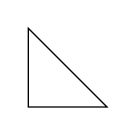
\begin{tikzpicture}
    \draw (0,0)--(1,0)--(0,1)--cycle;
\end{tikzpicture}のような形をしている.これを$[0,1]\times[0,1]$の形に変換したいので,$s=\xi,t=\frac{\eta}{1-\xi}$と変数変換する.
\end{tcolorbox}
$s=\xi,(1-s)t=\eta$と変数変換するとヤコビアンは$\begin{vmatrix}
    1 & 0 \\
    -t & 1-s
\end{vmatrix}=1-s$.
よって\begin{align}\int\int_{\xi+\eta+\zeta=1,\xi,\eta,\zeta\ge0} \xi^{\frac{1}{a}-1}\eta^{\frac{1}{b}-1}\zeta^{\frac{1}{c}-1} d\xi d\eta&=\int_0^1 \int_0^1 s^{\frac{1}{a}-1}(1-s)^{\frac{1}{b}-1}t^{\frac{1}{b}-1}(1-s)^{\frac{1}{c}-1}(1-t)^{{\frac{1}{c}-1}}(1-s)dsdt \\
    &=\int_0^1 s^{\frac{1}{a}-1}(1-s)^{\frac{1}{b}+\frac{1}{c}-1}ds\int_0^1 t^{\frac{1}{b}-1}(1-t)^{\frac{1}{c}-1}dt \\
    &=\Gamma\qty(\frac{1}{a})\Gamma\qty(\frac{1}{b}+\frac{1}{c})\Gamma\qty(\frac{1}{b})\Gamma\qty(\frac{1}{c})/ \Gamma\qty(\frac{1}{a}+\frac{1}{b}+\frac{1}{c})\Gamma\qty(\frac{1}{b}+\frac{1}{c})\\
    &=\frac{\Gamma\qty(\frac{1}{a})\Gamma\qty(\frac{1}{b})\Gamma\qty(\frac{1}{c})}{\Gamma\qty(\frac{1}{a}+\frac{1}{b}+\frac{1}{c})} 
\end{align}

よって$V=\frac{1}{abc}\frac{1}{\frac{1}{a}+\frac{1}{b}+\frac{1}{c}}\frac{\Gamma\qty(\frac{1}{a})\Gamma\qty(\frac{1}{b})\Gamma\qty(\frac{1}{c})}{\Gamma\qty(\frac{1}{a}+\frac{1}{b}+\frac{1}{c})}$.

\fbox{2}
(1) $G=H\cup K$と仮定する.
$x\in G\setminus H\subset K,y\in G\setminus K\subset H$に対して,$xy \in G = H \cup K$より$xy \in H$または$xy \in K$である.
$xy \in H$ならば$xy=h\in H$より,$x=yy^{-1}\in H$となり矛盾.
$xy \in K$ならば$xy=k\in K$より,$y=x^{-1}k\in K$となり矛盾.

(2) $x \in H\cap K, x \notin L$が存在すると仮定する.
$\ell \in G\setminus (H \cup K) \subset L$に対して,$x\ell \in H$なら$x\ell=h\in H$より$\ell=x^{-1}h\in H$となり矛盾.
$x\ell \in K$も同様.よって$x\ell \in L$だが,$\ell \in L$より$x\in L$となり矛盾.

\fbox{3}
$\Cl{A}$で$A$の閉包を表す.

$x\in U\cap V$に対して,$x\in B(x,r_x)\cap X \subset U\cap V$なる$r_x>0$が存在する.このとき,$x\in \Cl{B(x,r_x/2)} \cap X \subset U\cap V$である.
$x\in U\setminus V$についても$x\in \Cl{B(x,r_x/2)} \cap X \subset U$なる$r_x$が存在する.

$x\in V \setminus U$についても同様.

$r_x$を$x$に対して一つ固定する.

$\bigcup\limits_{x\in X} B(x,r_x/2) =X$であるから,コンパクト性より有限部分集合$X_0\subset X$が存在して$\bigcup\limits_{x\in X_0} B(x,r_x/2) =X$となる.

$X_{0,U} = \left\{ x\in X_0 \mid x_0 \in U \right\},X_{0,V} = \left\{ x\in X_0 \mid x_0 \in V \right\}$とする.
$K=\bigcup\limits_{x\in X_{0,U}} \Cl{B(x,r_x/2)} \cap X,L=\bigcup\limits_{x\in X_{0,V}} \Cl{B(x,r_x/2)} \cap X$とする.

$\Cl{B(x,r_x/2)}$は有界閉集合だからコンパクトで,$\Cl{B(x,r_x/2)} \cap X$も$X$のコンパクト集合である.
$K,L$は有限個のコンパクト集合の和集合だからコンパクトである.
$x \in X_{0,U}$に対して,$\Cl{B(x,r_x/2)} \cap X \subset U$であるから$K\subset U$.同様に$L\subset V$.

\fbox{4}行基本変形によって
$\begin{pmatrix}
    2 & 1 & 1  & 1 \\
    1 & t & t & 2t \\
    1 & t & t & t \\
\end{pmatrix}\rightarrow\begin{pmatrix}
    2 & 1 & 1  & 1 \\
    0 & 2t-1 & -1 & 3t-1 \\
    0 & 0 & 2t &  t\\
\end{pmatrix}$
とできる.
$t\neq0$ならさらに$\begin{pmatrix}
    4 & 2 & 0 & 1 \\
    0 & 4t-2 & 0 & 6t-1 \\
    0 & 0 & 2 &  1\\
\end{pmatrix}$である.

$f(t)=\det A(t)=2(2t-1)2t$であるから,$f(t_0)=0$ならば$t_0=1/2,0$である.
$t\to 1/2+0$のとき,$x(t)=\begin{pmatrix}
    -t/(2t-1) \\
    (6t-1)/(4t-2) \\
    1/2 
    \end{pmatrix}\rightarrow \begin{pmatrix}
        \infty \\
        \infty \\
        1/2
    \end{pmatrix}$である.
$t \to 1/2 -0$のとき,$x(t)\rightarrow \begin{pmatrix}
    -\infty \\
    -\infty \\
    1/2
\end{pmatrix}$である.

$t\rightarrow0$のとき,$x(t)\rightarrow \begin{pmatrix}
    0 \\
    1/2 \\
    1/2
\end{pmatrix}$である.




\end{document}